\documentclass[slides]{pgnotes}

\title{IRC deployment lab}

\begin{document}

\maketitle

\tableofcontents

\section{Aim}

We're going to draw together:

\begin{itemize}
\item Experience with Azure to date
\item Last year's experience with AWS
\item Basic SysAdmin and Networking knowledge
\end{itemize}

to put together a basic IRC server and demonstrate it with a Windows Client.

\subsection{Scenario}

\begin{center}
\includegraphics[width=0.75\linewidth]{scenario}
\end{center}


\section{Internet Relay Chat (IRC)}

Internet Relay Chat (IRC) is a chat-oriented text protocol running over port 6667.

\begin{itemize}
\item Originated in the 1980's
\item Still in use but popularity has waned:
  \begin{itemize}
  \item Social media, lack of ``rich content''.
  \item Not a simple 1-click setup
  \end{itemize}
\item Standardised protocol with choice of clients
  \begin{itemize}
  \item Easy to code up bots!
  \end{itemize}
\item Spartan interface with text commands like \texttt{/JOIN}
\item Insecure server defaults for authentication, channel creation etc.
\end{itemize}

At its most basic level an IRC server hosts a number of ``channels''.

\subsection{IRC server and clients}

\begin{center}
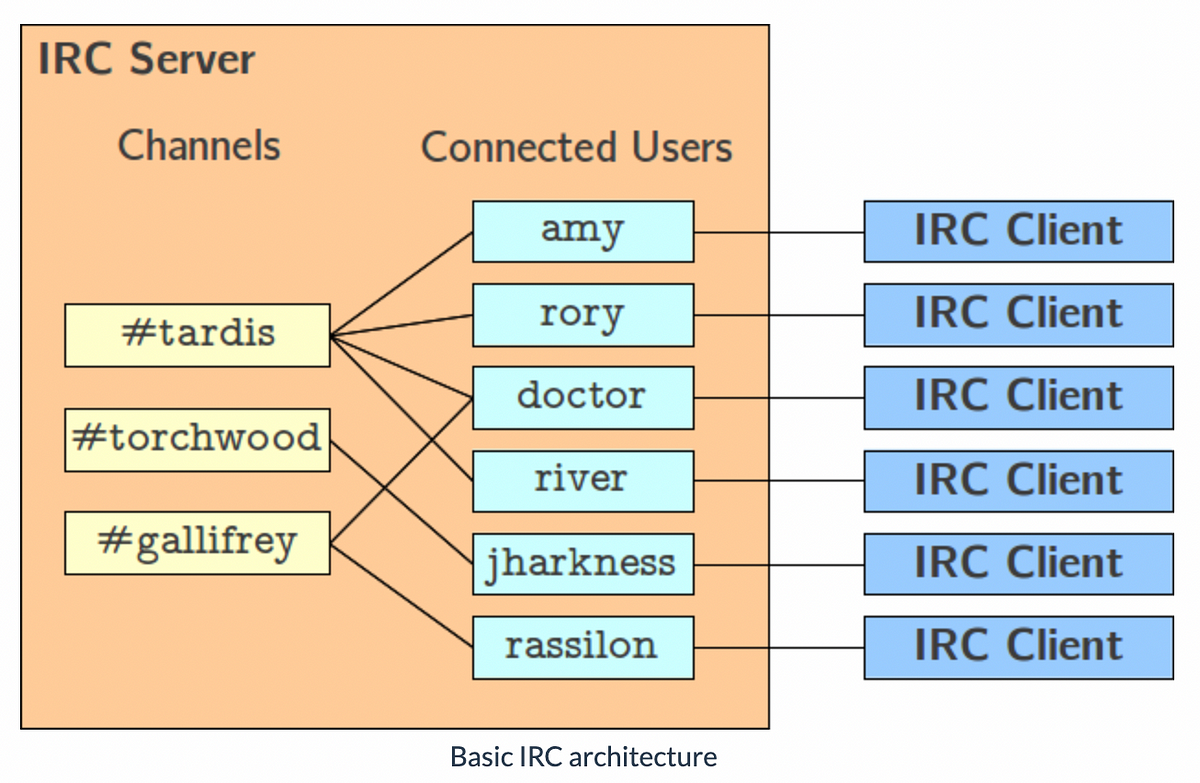
\includegraphics[width=0.6\linewidth]{basic_irc}
\end{center}


\subsection{Clients}

\begin{center}
  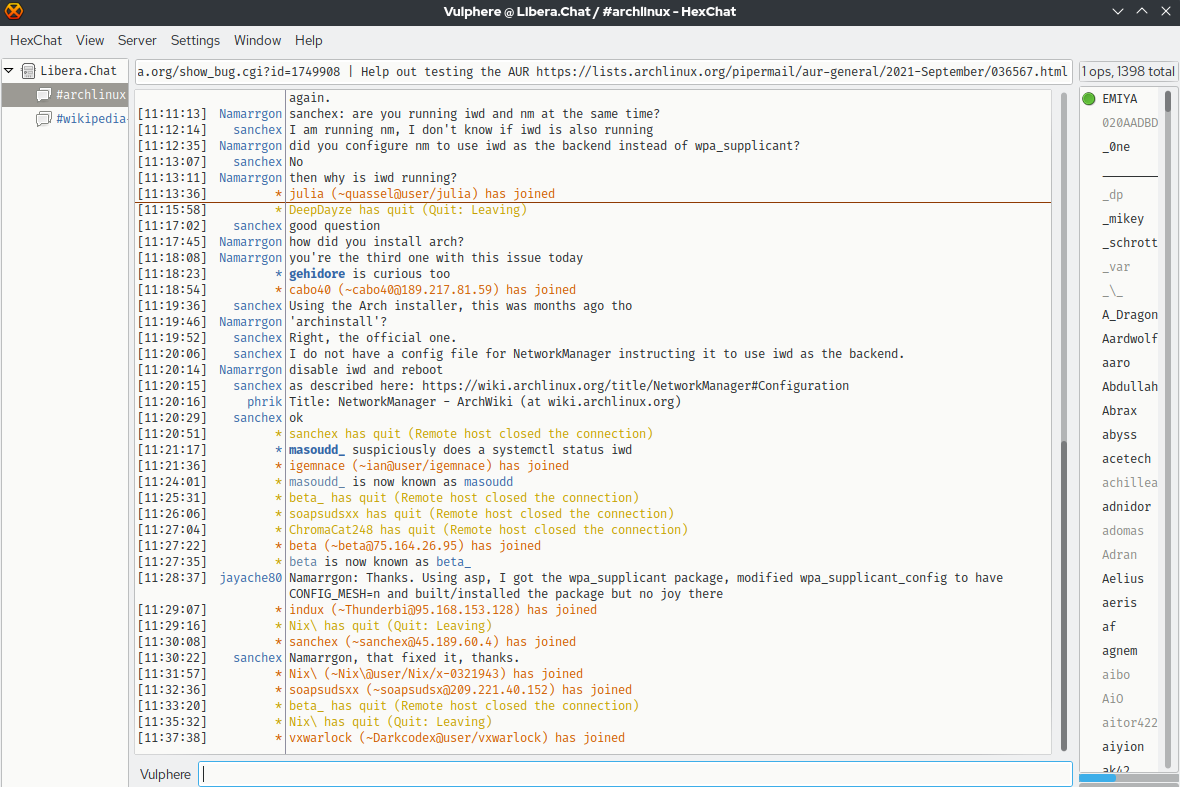
\includegraphics[width=0.6\linewidth]{hexchat}
\end{center}

\newpage
\subsubsection{Text-based clients}

\begin{center}
  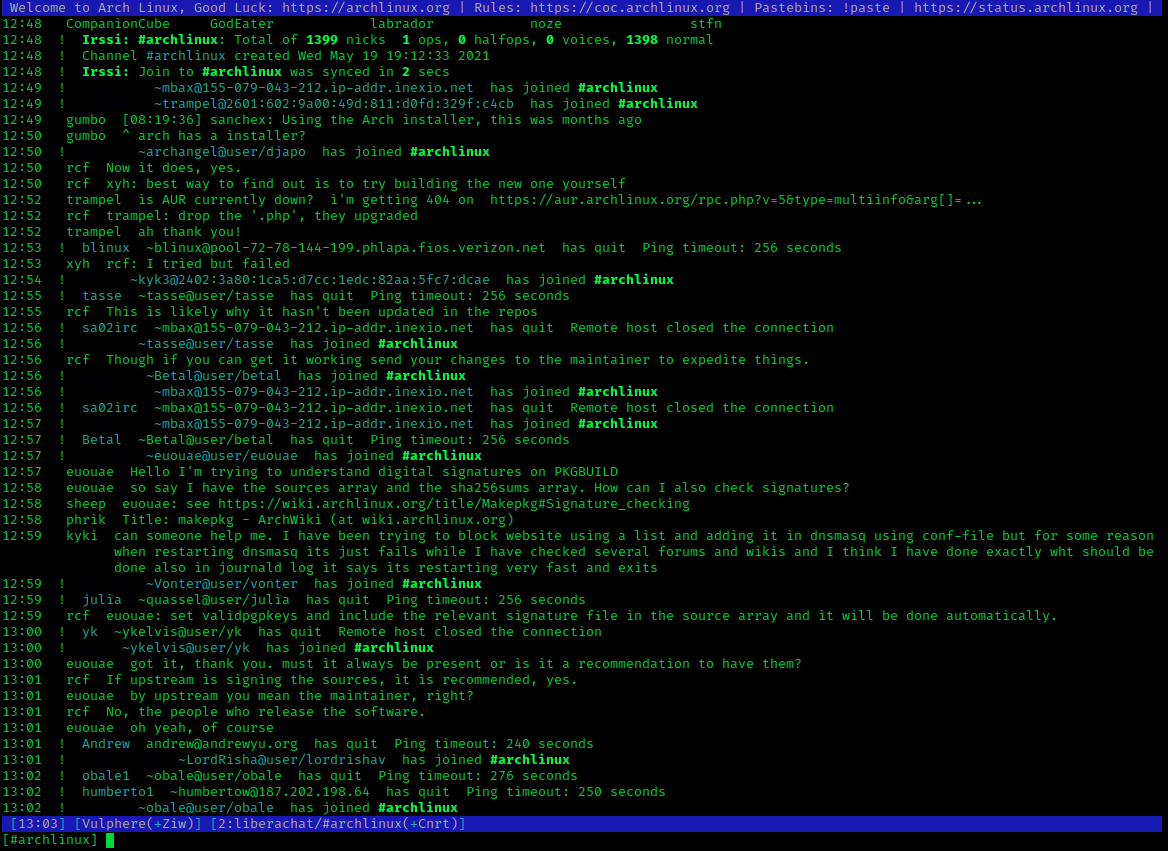
\includegraphics[width=0.5\linewidth]{irssi}
\end{center}


\subsection{Usage}

IRC has dwindled among the general public as a chat mechanism for a number of factors.

\begin{itemize}
\item Some open-source development communities still use it for commercial and political reasons.
\item Works very well on low-bandwidth connections (e.g. legacy satellite)
\item Development teams still use it sometimes in preference to Teams, Slack.
\item \textbf{Twitch} gaming streaming site employs it
\item Some monitoring systems use it for broadcast alterting and reporting
\end{itemize}

\newpage

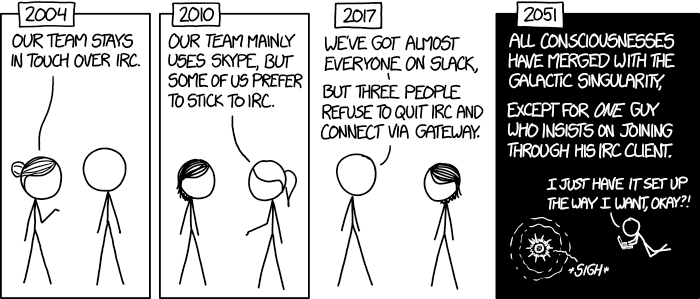
\includegraphics[width=1.0\linewidth]{xkcd_irc}


\section{SSH port forwarding}

IRC uses Port 6667.

We want to test an IRC client on our lab desktop connected to our Linux VM.

SSH forwarding is where SSH can \textbf{tunnel} a port from our local server through to the remote machine.

It's almost like a mini VPN and is \textit{VERY} useful!

\end{document}

